\documentclass[12pt]{article}

%fancy math symbols
\usepackage{amsmath}
\usepackage{amssymb}
\usepackage{cancel}

%fancy font
%\usepackage{pxfonts}
%\usepackage[T1]{fontenc}

%DAGs
\usepackage{tikz}
\usetikzlibrary{arrows,positioning,snakes,calc,shapes}
%\tikzset{>=latex}

\usepackage{bm}

%\newcolumntype{L}[1]{>{\raggedright\let\newline\\\arraybackslash\hspace{0pt}}p{#1}}

\usepackage{lineno}

%expectation operator
\usepackage{relsize}
\newcommand{\E}{\mathop{\vcenter{\hbox{\relsize{+1.1}$E$}}}}

\DeclareMathOperator{\logit}{logit}

%\usepackage[extra]{tipa}

\usepackage{color}
\usepackage{wrapfig}
\usepackage{indentfirst} % indents every paragraph
\usepackage{setspace} % ?
\usepackage[numbers,super,sort&compress]{natbib} % automate references

%USING REFERENCE PUNCTUATION FOR EPID STYLES WILL RETURN ERROR!!
%\bibpunct{}{}{,}{}{}{,} % Reference punctuation

\usepackage{booktabs} % for lines in table
\usepackage{rotating} % For sideways tables/figures
\usepackage[margin = .85in]{geometry} % allows to set margins. Use "vmargin" package to get different sized margins.
\usepackage{fancyhdr} %these three change the page number style from normal to "fancy".
\pagestyle{fancy}
\fancyhf{}
\usepackage{tabularx}
\usepackage{pdfpages}
\usepackage{longtable}
\renewcommand{\headrulewidth}{0pt} %default is to put a line at top. This command tells latex to make that line 0pt font (i.e., to remove it).
\pagenumbering{arabic} %arabic is the default. This command sets how page numbers appear. Capital "R" in Roman gives capital roman numerals. Lowercase "r" gives lowercase roman numerals. Good for toc, appendicies, etc. Alph/alph gives upper/lower case letters.
\usepackage{subfig}
\usepackage{mdwlist}
\usepackage{url}
\usepackage{verbatim}
\urlstyle{same}
\usepackage{multirow}
\usepackage{multicol}
\captionsetup[subfloat]{position = top, font = large} % For sub-figure captions
\usepackage[compact]{titlesec}
\usepackage[colorlinks = TRUE, urlcolor = blue, linkcolor = black, citecolor = black]{hyperref}
\usepackage{float}
\usepackage{xfrac}
\usepackage{lscape}
\usepackage{graphicx}
\begin{comment}
\newenvironment{myfig}[1]{%
 \refstepcounter{figure} \begin{center} \begin{minipage}[c]{.8\textwidth} \rule{\textwidth}{1pt} {\bf\large Figure \arabic{figure}: {#1}}\\  }{%
\rule{\textwidth}{1pt} \end{minipage} \end{center}}\renewcommand{\familydefault}{\sfdefault}
\end{comment}
\newcommand{\hl}[1]{\colorbox{yellow}{#1}}

%remove square brackets in bib
\makeatletter
\renewcommand\@biblabel[1]{#1.}
\makeatother


    \newcommand*\patchAmsMathEnvironmentForLineno[1]{%
      \expandafter\let\csname old#1\expandafter\endcsname\csname #1\endcsname
      \expandafter\let\csname oldend#1\expandafter\endcsname\csname end#1\endcsname
      \renewenvironment{#1}%
         {\linenomath\csname old#1\endcsname}%
         {\csname oldend#1\endcsname\endlinenomath}}%
    \newcommand*\patchBothAmsMathEnvironmentsForLineno[1]{%
      \patchAmsMathEnvironmentForLineno{#1}%
      \patchAmsMathEnvironmentForLineno{#1*}}%
    \AtBeginDocument{%
    \patchBothAmsMathEnvironmentsForLineno{equation}%
    \patchBothAmsMathEnvironmentsForLineno{align}%
    \patchBothAmsMathEnvironmentsForLineno{flalign}%
    \patchBothAmsMathEnvironmentsForLineno{alignat}%
    \patchBothAmsMathEnvironmentsForLineno{gather}%
    \patchBothAmsMathEnvironmentsForLineno{multline}%
    }

\usepackage{accents}
\newlength{\dhatheight}
\newcommand{\doublehat}[1]{%
    \settoheight{\dhatheight}{\ensuremath{\hat{#1}}}%
    \addtolength{\dhatheight}{-0.15ex}%
    \hat{\vphantom{\rule{1pt}{\dhatheight}}%
    \smash{\hat{#1}}}}

\newcolumntype{L}[1]{>{\raggedright\let\newline\\\arraybackslash\hspace{0pt}}p{#1}}

\def\linenumberfont{\normalfont\small\sffamily}

\rfoot{\thepage}
%\lfoot{Causal Inference in Social Epidemiology}
\rhead{EPID-2187}

\long\def\symbolfootnote[#1]#2{\begingroup%
\def\thefootnote{\fnsymbol{footnote}}\footnote[#1]{#2}\endgroup} 

\usepackage[symbol*]{footmisc}
\DefineFNsymbolsTM{myfnsymbols}{% def. from footmisc.sty "bringhurst" symbols
  \textdagger    \dagger
  \textdaggerdbl \ddagger
  \textsection   \mathsection
  \textbardbl    \|%
  \textparagraph \mathparagraph
}%
\setfnsymbol{myfnsymbols}

\usepackage{arydshln}
\usepackage{array}
\newcolumntype{L}[1]{>{\raggedright\let\newline\\\arraybackslash\hspace{0pt}}m{#1}}

\usepackage{lipsum}
\usepackage{wrapfig}

\usepackage{wasysym}
\begin{document}

\noindent {\Large Week 1: Basic Concepts in Survival Analysis}

\doublespacing
\normalfont

\vskip .5cm 

{\bf Instructions} (read carefully): 
\begin{itemize}
\item Each student must submit {\bf one} assignment as a .pdf file. **groups
\item Each member of the same group will receive the same grade. 
\item Please put the name of each group member on the first page. 
\item Use one inch margins and double spaced text. 
\item RMARKDOWN (Net file and rmd file) All of the R code for all applied questions must be provided as a separate file (with .R as the extension) along with the homework file.
\item This assignment is due {\bf electronically} through CANVAS on {\bf ..} at the beginning of class.
\end{itemize}

\vskip .5cm 

\noindent {\bf Question 1)} Using the language of "censoring" and/or "truncation" (left, right, and/or interval), explain why a prospective cohort study is often seen as higher quality than a retrospective cohort study.

\noindent {\bf Question 2)} Using Figure 1, draw the line diagram for for ID = 0 that would result if this individual was left truncated.

\begin{figure*}
	\caption{Line diagram with six hypothetical individuals who enter into a study at age 46 and who exit at age 56.}
	\center
	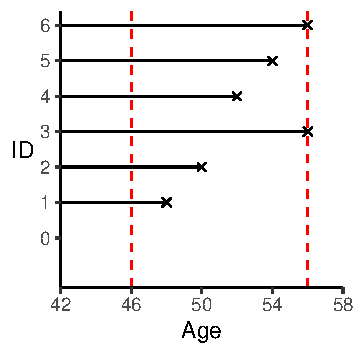
\includegraphics[scale=1]{../../figures/2021_12_08-hw-fig.pdf}
\end{figure*}

\noindent {\bf Question 3)} Please do a basic exploratory analysis of the "example\_dat1.csv" dataset. No more than 1/2 page. Provide results for the exposure, the confounder, and the outcome.

\noindent {\bf Question 4)} Describe, in words, the interpretation of the CDF: 
$$F(t) = P(T \leq t)$$

AND the survival function:

$$S(t) = P(T > t)$$

if $T$ represents age at death from all causes, and $t$ represents 64 years of age.

\noindent {\bf Question 5)} Using the first five observations from the synthetic data in Table 1 of the course notes, write out the terms for the Kaplan-Meier estimator $\hat{S}(t) = \prod_{k \in t_k \leq t} (1 - d_k/n_k)$.

\noindent {\bf Question 6)} Fit the `survfit()` function to the "example\_dat1.csv" data. Examine the R object that you get from this fit. Is there enough information in this object for you to determine the median survival time for the outcome? If so, what is the median survival time.

\noindent {\bf Question 7)} Using "example\_dat1.csv", plot the cumulative distribution function using the KM estimator. Interpret the curve.

\end{document}	

